\chapter{Agricultura}
\section{Introdução}
\par A agricultura tem uma máxima importância para a economia brasileira, e por consequência também é importante para os estados brasileiros. O agronegócio representou 21,4\% do PIB nacional em 2019, demonstrando o quão providencial é para o nosso país. Já para o Tocantins, sua participação está abaixo da média nacional, pois o agronegócio está abaixo de 15\% da representação do PIB estadual. Nesta sessão do Boletim iremos apresentar os seguintes dados da agricultura; Área de produção, colhida, produção de cereais e oleaginosas e o seu rendimento médio. Em outra parte iremos analisar os dados de abates de animais, produção de ovos de galinha e leite. 
\\
Nas páginas a seguir iremos analisar os dados mais relevantes para o agronegócio estadual e para a nossa conjuntura do trimestre, sabe-se que uma análise total das cadeias produtivas da agricultura requerem estudos mais aprofundados. Aqui, iremos apresentar e analisar os dados de mais relevância por produção e participação no cenário econômico.

\begin{smbox}[label={labelbox},nameref={Agricultura}]{Agricultura em geral}
No Brasil existem inúmeros órgãos que cuidam e divulgam dados sobre agricultura, sejam municipais, estaduais ou federativo. Uma referencia impar destes dados é o SIDRA (Sistema IBGE de Recuperação Automática). Outra referência interessantisima para agricultura é o IPEA (Instituto de Pesquisa Econômica Aplicada), além das secretarias estaduais e municipais que realizam pesquisas próprias, no estado tocantinense a FIETO-TO e a secretaria da fazenda realizam pesquisas similares.
\end{smbox}

\section{Produção}
\par O estado do Tocantins apresentou no primeiro semestre de 2020 uma produção no tamanho equivalente a 1.520.698 hectares. Dentre os 5 principais produtos plantados no estado, destaca-se as elevadas quantidades providas da cana-de-açúcar e soja, responsáveis por 38.2\% e 36.2\% do total produzido, seguido pelo milho como o terceiro produto mais cultivado no estado neste período correspondendo à 14.5\%. A produção de arroz e mandioca também ganha destaque ao representar um montante de 8.2\% e 3\% respectivamente, fechando assim o ranking dos cinco produtos com maior influência na agricultura tocantinense. 

\begin{figure}[h]
	\caption{Produção - Tocantins 2020}
	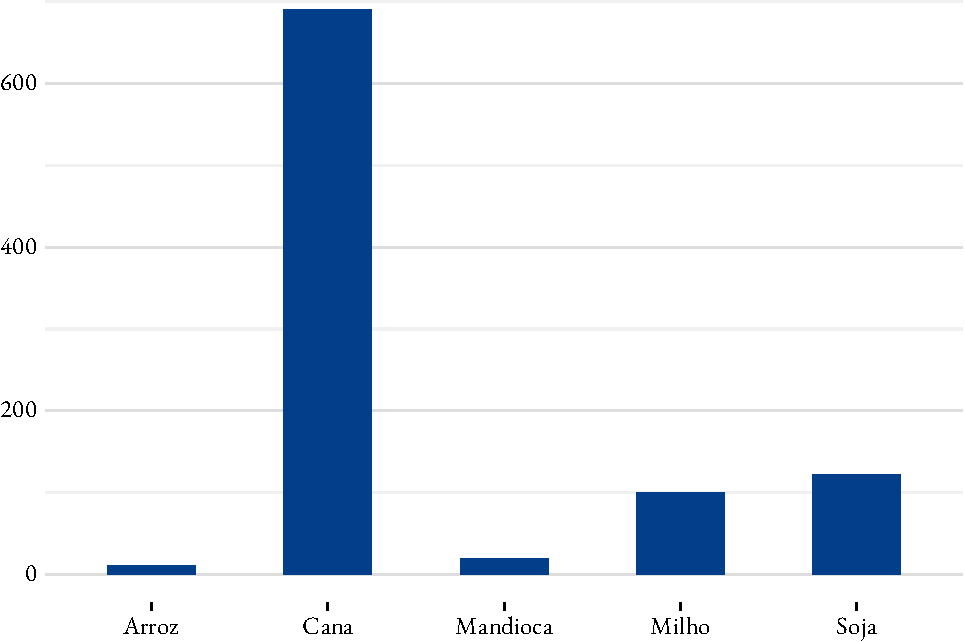
\includegraphics{fig/producao-1.pdf}
	\source{IBGE/SIDRA}
	\notes{Produção por toneladas dos maiores produtos tocantinenses}
\end{figure}

\begin{smbox}[label={labelbox},nameref={Agricultura}]{Produção em evidência}
	O Estado tocantinense tem uma economia pautada no agronegócio (não apenas a do Tocantins, a brasileira em si) e com as frequentes desvalorizações do nosso câmbio torna-se atrativo demais produzir uma commodity como a Soja. E por isso, vemos que no estado do Tocantins a Soja é tão exponencial assim, como falado na sessão de balanços de pagamentos, o valor que esse produto gera ao estado é absurdo e crucial para a economia.
\end{smbox}

\section{Rendimento Médio}
\par Dentre os cinco principais produtos cultivados na agricultura tocantinense, o rendimento médio mostra como as características próprias de cada um deles tem resultado determinante no cálculo da área que deve ser plantada, visando a quantidade em que será colhida. O cálculo é feito pela divisão entre quilogramas colhidos pela área plantada, significando que, quanto maior o valor do rendimento médio, menor é a área necessária para sua colheita. Sendo assim, os dados mostram que o maior rendimento médio entre estes produtos é da cana-de-açúcar, chegando ao elevado valor de 70.7\%. O segundo produto é a mandioca, com um rendimento médio de 14..3\%, seguido pelo milho, ao total de 7.7\%, arroz, com 4.7\% e por fim, a soja, com um rendimento médio de 2.6\%, ou seja, precisando então de uma vasta área plantada para colher sua quantidade desejada. 

\begin{figure}[h]
	\caption{Rendimento médio - Tocantins 2020}
	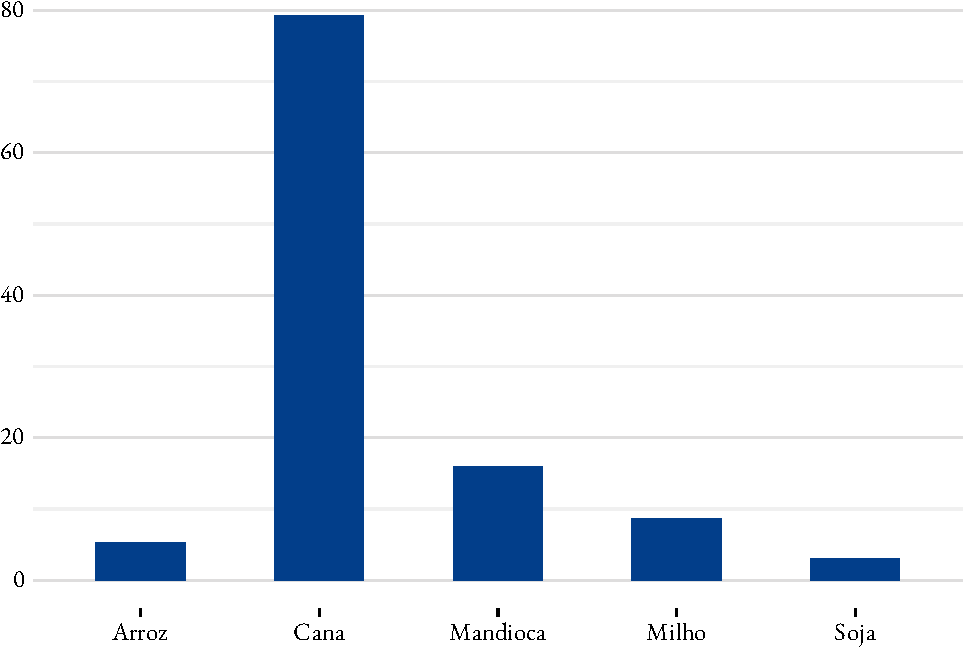
\includegraphics{fig/rendim_medio-1.pdf}
	\source{IBGE/SIDRA}
\end{figure}

\section{Áreas plantadas e colhidas}

\par Baseando-se no primeiro semestre temos os dados das áreas plantadas e colhidas e consequentemente, os cereais e oleaginosas que mais usam o espaço tocantinense para a produção. No primeiro semestre de 2020, o Tocantins utilizou-se de 1.427.342 hectares para plantação. O maior espaço disso é para a Soja que utilizou-se de 975.513 hectares para a produção, demonstrando que a Soja requer de um bom espaço para o seu cultivo. Numa visão total desta área toda a Soja tem 68.7\% de utilização do espaço de plantio, em seguida vem o milho que utiliza 18.8\% do território, os dois espaços mais usado para a plantação. O arroz corresponde 8.8\%, em seguida cana com 2.7\% e mandioca com 1\%.
\\
A soja utiliza-se de um território enorme para se ter uma produtividade alta, diferentemente da cana-de-açúcar que tem uma alta produtividade por hectare, já exposta acima pelos dados de rendimento médio.
\begin{figure}[h]
	\caption{Área Plantada - Tocantins 2020}
	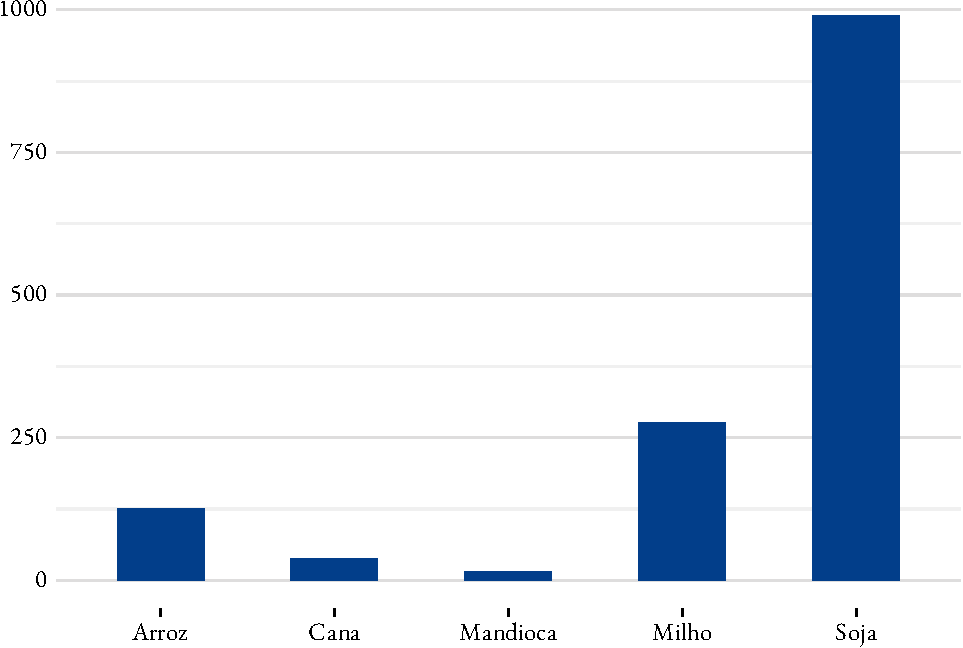
\includegraphics{fig/area_plantada-1.pdf}
	\source{IBGE/SIDRA}
	\notes{Relação por trimestre a partir do 1T de 2019 para acompanhar o movimento que os empregos estão tendo.}
\end{figure}

\section{Produção de leite}
\par O Tocantins é conhecido pela sua produção agropecuária, com foco na produção de Soja e seus derivados. Por em parte da sua produção fica com Leite, o estado do Tocantins no ano de 2019 produziu 132.237(Mil Litros), apesar de uma produção grande, o estado ainda não se tornou referência no segmento ficando com menos de 1 percentual na produção do Brasil. O estado mantém valores constantes na sua produção, e não apresenta grande variação nos últimos cinco trimestres. Por fim, sua produção no primeiro trimestre do ano de 2020 teve uma produção de 37.273 Mil Litros, apresentando um aumento pequeno comparado ao valor do quarto semestre de 2019 que teve uma produção de 36369. 
\\
\begin{figure}[h]
	\caption{Produção de Leite - Tocantins 2020}
	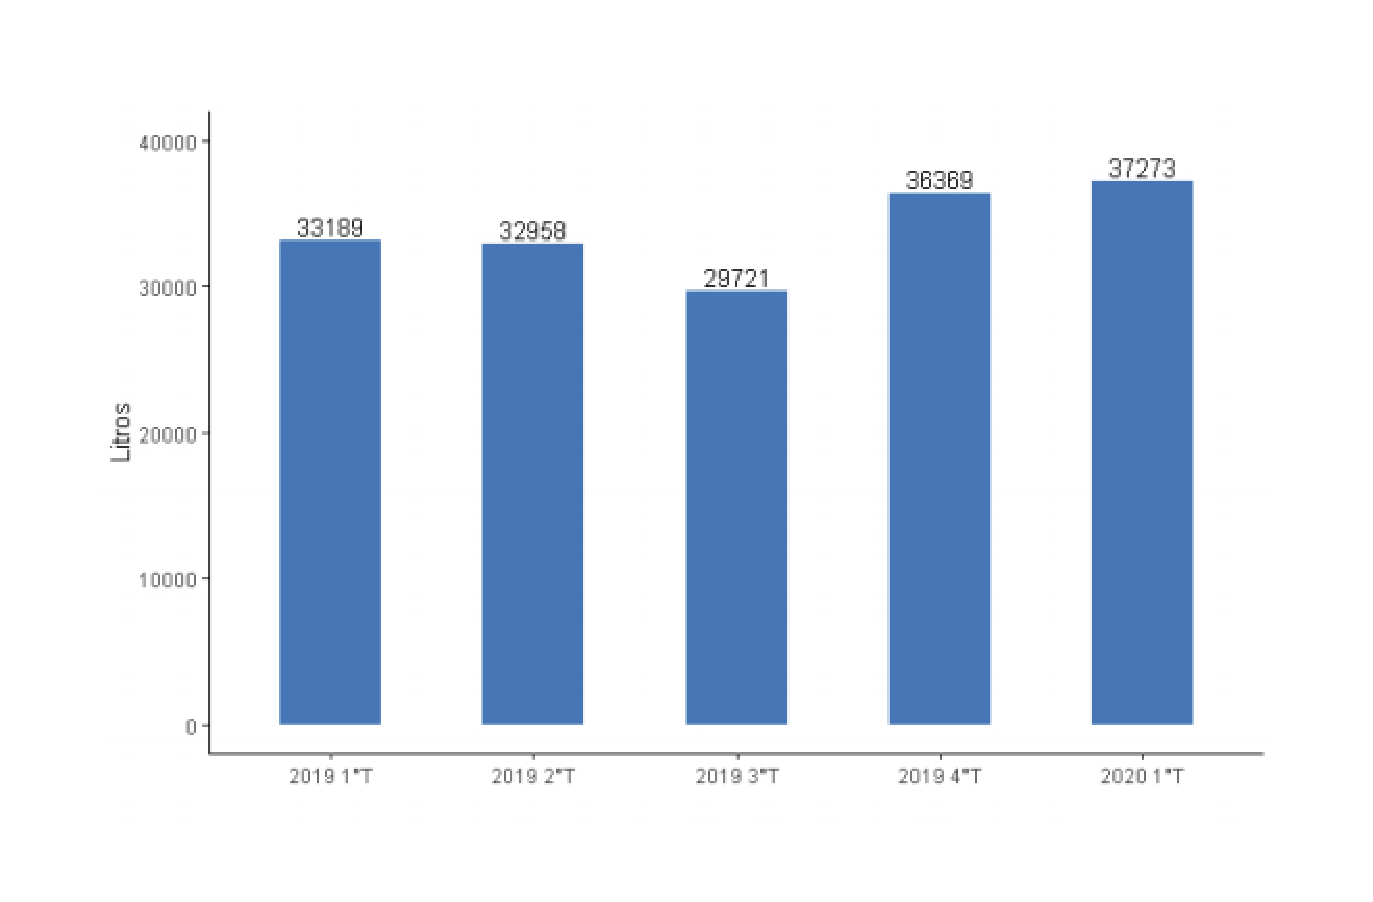
\includegraphics[width=\linewidth]{fig/Produção de leite.pdf}
	\source{IBGE/SIDRA}
	\notes{Relação por trimestre a partir do 1T de 2019 para acompanhar o movimento que os empregos estão tendo.}
\end{figure}

\section{Abate de animais}

\par No quarto trimestre de 2019 os frigoríficos suspenderam abate no Tocantins após o governo cortar incentivos fiscais. Os pecuaristas e empresários do setor sentiram o impacto após o corte do benefício, que era a isenção do imposto sobre circulação de mercadorias e serviços (ICMS) para o setor. A alíquota passou a ser de 12\% foi uma das consequências que fez subir o preço da carne para esse ano de 2020.


\begin{figure}[h]
	\caption{Abate de animais - Tocantins}
	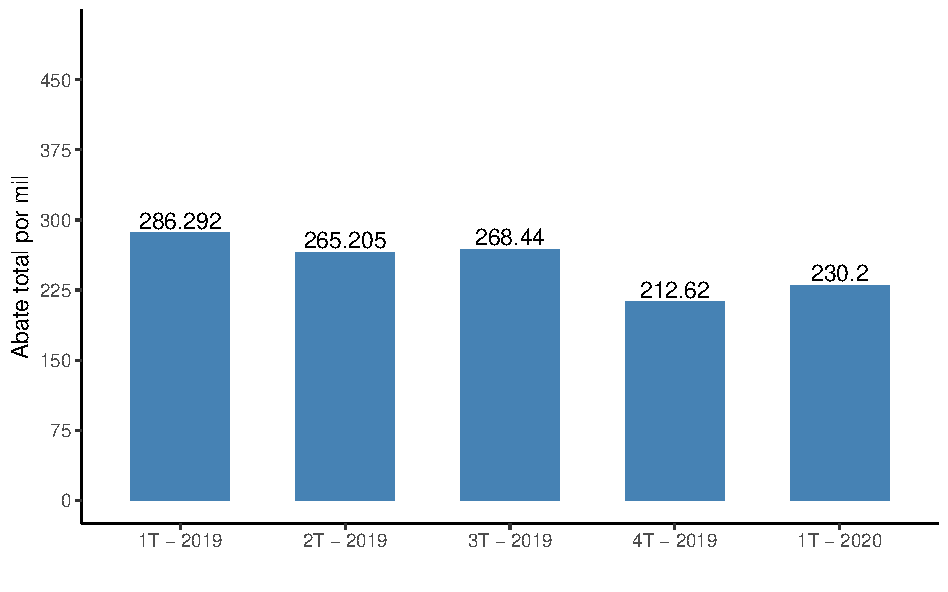
\includegraphics[width=\linewidth]{fig/Abate de animais.pdf}
	\source{Ministério do Trabalho}
	\notes{Relação do primeiro trimestre de 2020 por setores.}
\end{figure}

\par O gráfico acima mostra o abate total de animais com uma queda no quarto trimestre de 2019 que foi acarretada pela isenção do incentivo fiscais para o abate dos animais no frigorífico no Tocantins. 

\begin{figure}[h]
	\caption{Dados sobre o abate no primeiro trimestre - Tocantins 2020}
	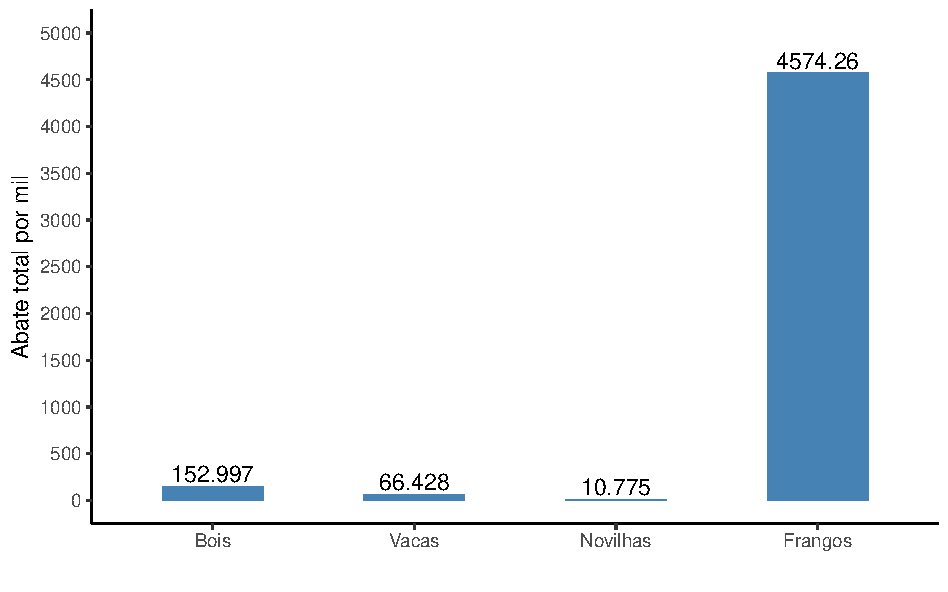
\includegraphics[width=\linewidth]{fig/Abate 1T.pdf}
	\source{IBGE/SIDRA}
	\notes{Relação por trimestre a partir do 1T de 2019 para acompanhar o movimento que os empregos estão tendo.}
\end{figure}

\par Enquanto alguns setores da economia são prejudicados pela crise econômica de 2020 gerada pelo vírus COVID-19. O setor do Agro se reinventa e expande sua produção em frangos, a empresa Grupo goiano SSA Alimentos, dona das marcas “SuperFrango” e “Boua”, esteve no estado no ano de 2019 para conhecer incentivos que o estado oferece para esse setor. A empresa mantém uma distribuidora em Paraíso do Tocantins, mas tem interesse em instalar um complexo industrial para abate de frangos no Estado devido aos incentivos do estado serem bons. \\
Esses incentivos fizeram com que o abate de frangos ter aumentado no estado, como é demonstrado pelo gráfico acima.

\section{Abate de frangos, bovinos, vacas e novilhas}

\par Já nesse setor de animais, iremos expor alguns dados referentes aos abates dessas categorias.

\begin{figure}[h]
	\caption{Abate de bois, frangos, novilhas e vacas}
	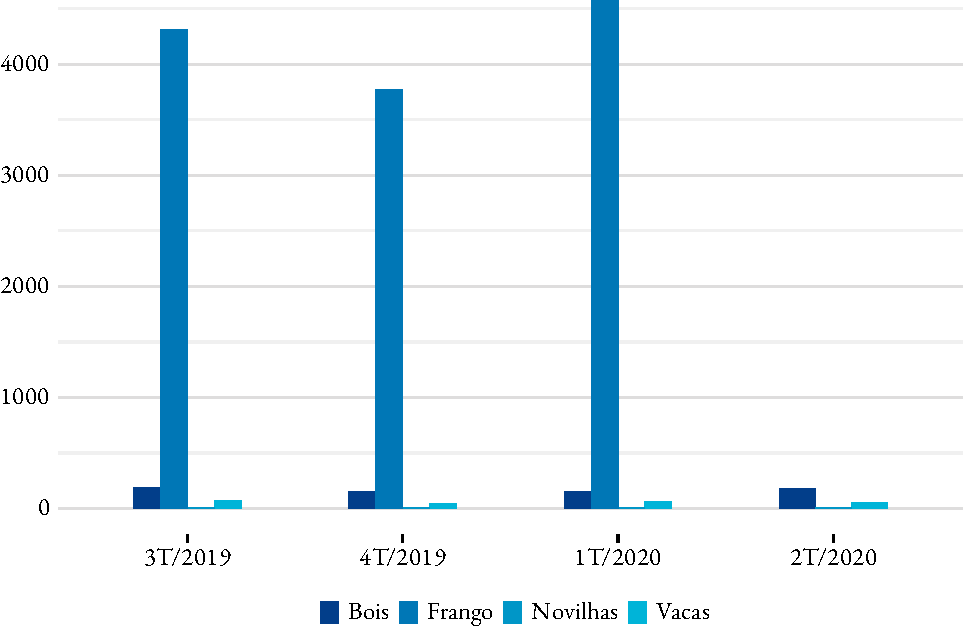
\includegraphics{fig/abates-1.pdf}
	\source{IBGE/SIDRA}
\end{figure}
	

\section{Ovos de galinha}

\begin{figure}[h]
	\caption{Total de galinhas poedeiras - Tocantins}
	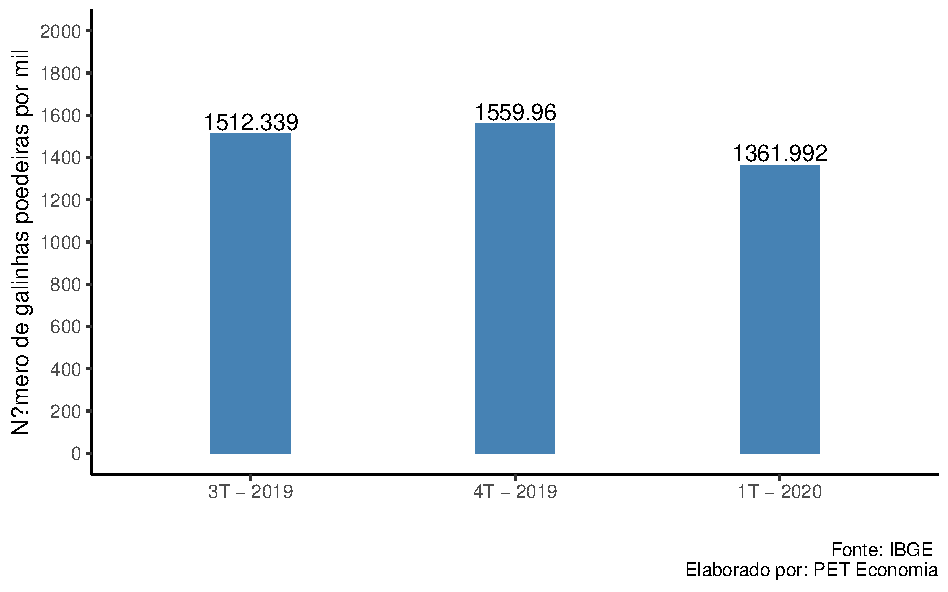
\includegraphics[width=\linewidth]{fig/Ovos.pdf}
	\source{IBGE/SIDRA}
	\notes{Relação por trimestre a partir do 1T de 2019 para acompanhar o movimento que os empregos estão tendo.}
\end{figure}

\begin{figure}[h]
	\caption{Quantidades de ovos de galinha produzida - Tocantins}
	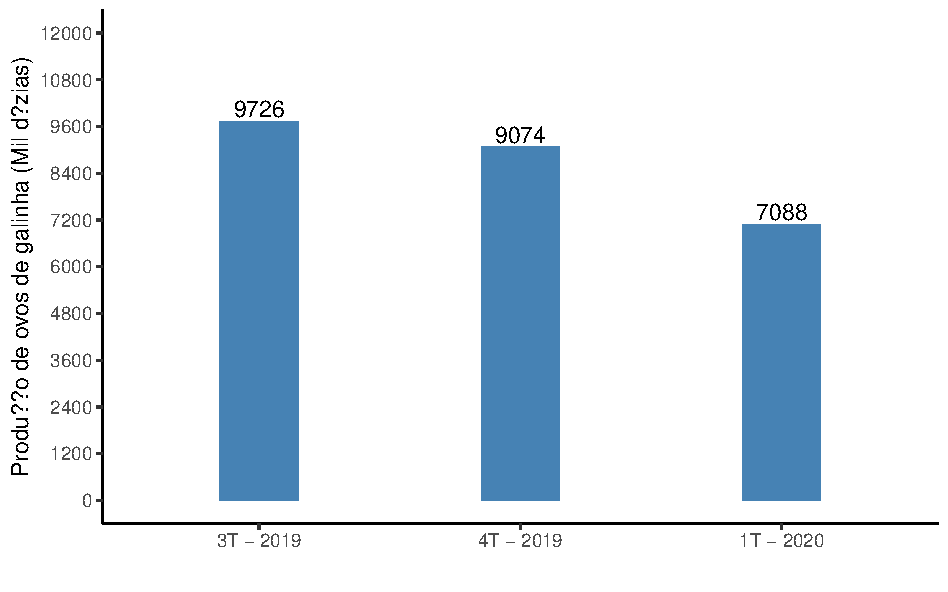
\includegraphics[width=\linewidth]{fig/Ovos produzido.pdf}
	\source{IBGE/SIDRA}
	\notes{Relação por trimestre a partir do 1T de 2019 para acompanhar o movimento que os empregos estão tendo.}
\end{figure}

